\section{Questions \& Discussion}

\begin{frame}
\frametitle{Key Takeaways}

\begin{conceptbox}{Rasterization Philosophy}
\begin{itemize}
    \item \textbf{Speed over Accuracy}: Fast approximations for real-time rendering
    \item \textbf{Hardware Optimization}: Specialized units for common operations
    \item \textbf{Clever Approximations}: Z-buffer, perspective-correct interpolation
    \item \textbf{Parallelism}: Massive parallel processing for fragments
\end{itemize}
\end{conceptbox}

\begin{mathbox}{Modern Pipeline Benefits}
\begin{itemize}
    \item \textbf{Programmability}: Flexible shaders for custom effects
    \item \textbf{Efficiency}: Fixed-function units for performance-critical stages
    \item \textbf{Scalability}: Works across different hardware configurations
    \item \textbf{Compatibility}: Backward compatibility with legacy content
\end{itemize}
\end{mathbox}

\end{frame}

\begin{frame}
\frametitle{Discussion Questions}

\begin{enumerate}
    \item \textbf{Trade-offs}: When would you choose rasterization over ray tracing? What factors influence this decision?
    
    \vspace{0.3cm}
    
    \item \textbf{Pipeline Design}: Why is the graphics pipeline designed with both programmable and fixed-function stages?
    
    \vspace{0.3cm}
    
    \item \textbf{Optimization}: Given a scene with 1 million triangles, what optimization strategies would you employ?
    
    \vspace{0.3cm}
    
    \item \textbf{Future Trends}: How might rasterization evolve with advances in GPU architecture?
    
    \vspace{0.3cm}
    
    \item \textbf{Memory Hierarchy}: How does understanding GPU memory hierarchy inform shader optimization?
\end{enumerate}

\end{frame}

\begin{frame}
\frametitle{Rasterization vs Ray Tracing}

\begin{center}
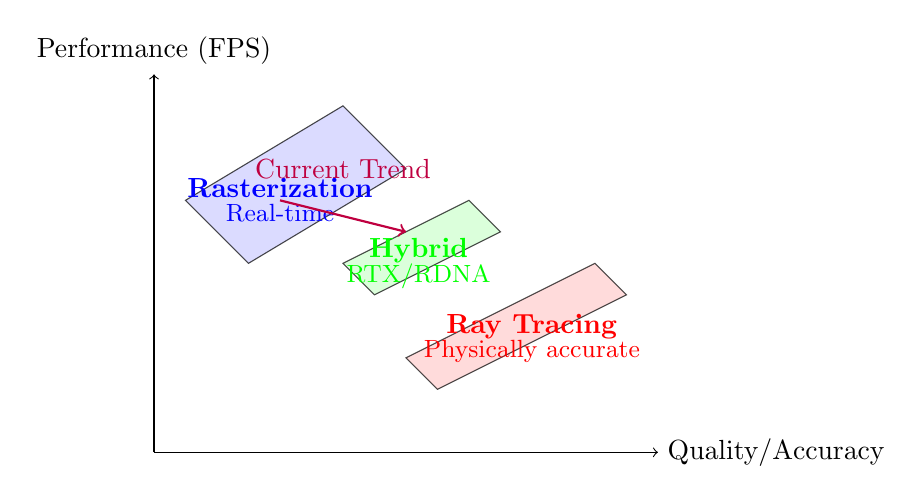
\begin{tikzpicture}[scale=0.8]
    % Performance vs Quality graph
    \draw[->] (0,0) -- (8,0) node[right] {Quality/Accuracy};
    \draw[->] (0,0) -- (0,6) node[above] {Performance (FPS)};
    
    % Rasterization region
    \draw[fill=blue!20, opacity=0.7] (0.5,4) -- (3,5.5) -- (4,4.5) -- (1.5,3) -- cycle;
    \node[blue] at (2,4.2) {\textbf{Rasterization}};
    \node[blue] at (2,3.8) {\small Real-time};
    
    % Ray tracing region  
    \draw[fill=red!20, opacity=0.7] (4.5,1) -- (7.5,2.5) -- (7,3) -- (4,1.5) -- cycle;
    \node[red] at (6,2) {\textbf{Ray Tracing}};
    \node[red] at (6,1.6) {\small Physically accurate};
    
    % Hybrid region
    \draw[fill=green!20, opacity=0.7] (3.5,2.5) -- (5.5,3.5) -- (5,4) -- (3,3) -- cycle;
    \node[green] at (4.2,3.2) {\textbf{Hybrid}};
    \node[green] at (4.2,2.8) {\small RTX/RDNA};
    
    % Current trend arrow
    \draw[->, thick, purple] (2,4) -- (4,3.5);
    \node[purple] at (3,4.5) {Current Trend};
\end{tikzpicture}
\end{center}

\begin{conceptbox}{The Future: Hybrid Approaches}
\begin{itemize}
    \item \textbf{RT Reflections}: Ray traced reflections with rasterized primary rays
    \item \textbf{RT Shadows}: Ray traced shadows for accurate lighting
    \item \textbf{RT Global Illumination}: One-bounce global illumination
    \item \textbf{Variable Rate Shading}: Adaptive quality based on importance
\end{itemize}
\end{conceptbox}

\end{frame}

\begin{frame}
\frametitle{Hands-on Exploration}

\begin{mathbox}{Practical Exercises}
\begin{enumerate}
    \item \textbf{Pipeline Visualization}: Use RenderDoc or similar tools to analyze a frame
    \item \textbf{Shader Profiling}: Measure vertex vs fragment shader performance
    \item \textbf{Memory Optimization}: Implement texture compression and LOD systems
    \item \textbf{Draw Call Batching}: Optimize a scene with many small objects
\end{enumerate}
\end{mathbox}

\begin{conceptbox}{Tools for Learning}
\begin{itemize}
    \item \textbf{Graphics Debuggers}: RenderDoc, NSight Graphics, Radeon GPU Profiler
    \item \textbf{Engines}: Unity, Unreal Engine (study their renderers)
    \item \textbf{APIs}: OpenGL, Direct3D, Vulkan, Metal
    \item \textbf{Frameworks}: Three.js, WebGL for web-based experimentation
\end{itemize}
\end{conceptbox}

\end{frame}

\begin{frame}
\frametitle{Open Discussion}

\begin{center}
\Large{\textbf{Questions?}}

\vspace{1cm}

\textit{"The best way to learn graphics is to implement it yourself."}

\vspace{1cm}

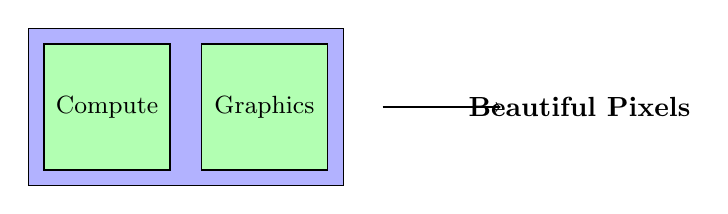
\begin{tikzpicture}
    % Simple GPU icon
    \draw[fill=blue!30] (0,0) rectangle (4,2);
    \draw[fill=green!30] (0.2,0.2) rectangle (1.8,1.8);
    \draw[fill=green!30] (2.2,0.2) rectangle (3.8,1.8);
    
    \node at (1,1) {\small Compute};
    \node at (3,1) {\small Graphics};
    
    \draw[->] (4.5,1) -- (6,1);
    \node at (7,1) {\textbf{Beautiful Pixels}};
\end{tikzpicture}
\end{center}

\end{frame}
